\documentclass[aspectratio=43,10pt]{beamer}

% =============================================================================
% PPD-II SECOND REVIEW PRESENTATION
% Title: AI-Powered Security Operations Center (SOC) Assistant Using Large Language Models
% Student: Kunal Sanga (2301341031) | Supervisor: Miss Alka Dash
% Institution: Silicon Institute of Technology, Sambalpur
% Template: Custom Silicon Institute of Technology Beamer Design (SKP-beamer compatible)
% Compile with: pdfLaTeX in Overleaf or local TeX distribution
% =============================================================================

\usepackage[utf8]{inputenc}
\usepackage[T1]{fontenc}
\usepackage{lmodern}
\usepackage{graphicx}
\usepackage{xcolor}
\usepackage{tikz}
\usetikzlibrary{calc,positioning,arrows.meta,shadows,fit,shapes.geometric}
\usepackage{booktabs}
\usepackage{colortbl}
\usepackage{tabularx}
\usepackage{array}
\usepackage{ragged2e}
\usepackage{tcolorbox}
\tcbuselibrary{skins}

% --- Color Palette Aligned with Template Visual Identity ---
\definecolor{SOCteal}{RGB}{17,94,119}          % Deep academic teal
\definecolor{SOCtealLight}{RGB}{53,145,160}    % Cyan accent
\definecolor{SOCnav}{RGB}{64,64,64}            % Dark gray navigation strip
\definecolor{SOCdark}{RGB}{19,51,72}           % Midnight dark text
\definecolor{SOCpale}{RGB}{237,243,247}        % Soft card background
\definecolor{SOCline}{RGB}{207,219,225}        % Card border
\definecolor{SOCgray}{RGB}{93,108,118}         % Muted gray
\definecolor{SOCwhite}{RGB}{255,255,255}
\definecolor{SOCgreen}{RGB}{34,139,74}         % Passing / Verified
\definecolor{SOCamber}{RGB}{210,105,30}        % Pending / Warning

\usetheme{default}
\setbeamersize{text margin left=0.065\paperwidth,text margin right=0.065\paperwidth}
\setbeamerfont{normal text}{size=\small}
\setbeamercolor{normal text}{fg=SOCdark,bg=white}
\setbeamercolor{structure}{fg=SOCteal}
\setbeamercolor{itemize item}{fg=SOCteal}
\setbeamercolor{itemize subitem}{fg=SOCtealLight}
\setbeamertemplate{navigation symbols}{}
\setbeamertemplate{itemize item}{\raisebox{0.15ex}{\tiny$\blacktriangleright$}}
\setbeamertemplate{itemize subitem}{\raisebox{0.15ex}{\tiny$\blacktriangleright$}}

% Top progress navigation strip
\newcommand{\SOCnavstrip}{%
\begin{tikzpicture}[remember picture,overlay]
  \fill[SOCnav] (current page.north west) rectangle ([yshift=-0.34cm]current page.north east);
  \node[anchor=north west,inner sep=0pt,font=\fontsize{4.6}{5.2}\selectfont,text=white] 
    at ([xshift=0.12cm,yshift=-0.06cm]current page.north west)
    {Problem\quad Scope\quad [1] System Design\quad Data Flow\quad [2] Implementation\quad Frontend\quad Testing\quad [3] Tech Approach\quad Evaluation\quad [4] Results\quad Limitations\quad Conclusion};
  \node[anchor=north west,inner sep=0pt,font=\fontsize{4.6}{5.2}\selectfont,text=white] 
    at ([xshift=0.12cm,yshift=-0.20cm]current page.north west)
    {$\bullet\quad\bullet\quad\bullet\bullet\quad\bullet\bullet\quad\bullet\bullet\quad\bullet\bullet\quad\bullet\bullet\quad\bullet\bullet\quad\bullet\bullet\quad\bullet\bullet\quad\bullet\quad\bullet$};
\end{tikzpicture}%
}

% Footer strip
\newcommand{\SOCfooter}[1]{%
\begin{tikzpicture}[remember picture,overlay]
  \fill[SOCnav] (current page.south west) rectangle ([yshift=0.28cm]current page.south east);
  \node[anchor=west,text=white,font=\fontsize{5.5}{6}\selectfont]
    at ([xshift=0.12cm,yshift=0.14cm]current page.south west)
    {Silicon Institute of Technology, Sambalpur};
  \node[anchor=center,text=white,font=\fontsize{5.5}{6}\selectfont]
    at ([yshift=0.14cm]current page.south)
    {AI-Powered SOC Assistant \quad\textbar\quad PPD-II Second Review};
  \node[anchor=east,text=white,font=\fontsize{5.5}{6}\selectfont]
    at ([xshift=-0.70cm,yshift=0.14cm]current page.south east)
    {October 2026};
  \node[anchor=east,text=white,font=\fontsize{5.5}{6}\selectfont]
    at ([xshift=-0.10cm,yshift=0.14cm]current page.south east)
    {#1 / 15};
\end{tikzpicture}%
}

% Header bar with logo
\newcommand{\SOCheading}[2]{%
\begin{tikzpicture}[remember picture,overlay]
  \fill[SOCteal] (current page.north west) rectangle ([yshift=-0.72cm]current page.north east);
  \node[anchor=west,text=white,font=\sffamily\fontsize{13}{15}\bfseries\selectfont]
    at ([xshift=0.25cm,yshift=-0.28cm]current page.north west) {#1};
  \node[anchor=west,text=SOCpale!90,font=\sffamily\fontsize{7.5}{9}\selectfont]
    at ([xshift=0.25cm,yshift=-0.54cm]current page.north west) {#2};
  \node[anchor=east] at ([xshift=-0.25cm,yshift=-0.36cm]current page.north east) {
    \IfFileExists{sitlogo.png}{
\includegraphics[height=0.48cm]{sitlogo.png}}{}
  };
\end{tikzpicture}%
}

% Standard slide wrapper
\newcommand{\SOCslide}[3]{%
\begin{frame}[plain]
\SOCnavstrip
\SOCheading{#1}{#2}
\vspace*{0.38cm}
#3
\SOCfooter{\thepage}
\end{frame}
}

% Card component with top colored accent rule
\newcommand{\SOCcard}[3]{%
\begin{tikzpicture}
\node[
  draw=SOCline,fill=SOCpale,rounded corners=2pt,
  line width=0.45pt,top color=SOCpale,bottom color=white,
  text width={\dimexpr#1-12pt\relax},inner sep=6pt,align=left,
  drop shadow={opacity=.10,shadow xshift=1pt,shadow yshift=-1pt}
] (card) {\textbf{\color{SOCdark}#2}\\[2pt]\small #3};
\draw[SOCteal,line width=2pt] (card.north west)--(card.north east);
\end{tikzpicture}%
}

% Colored highlight box
\newcommand{\SOCbox}[4]{%
\begin{tikzpicture}
\node[
  draw=#2,fill=#3,rounded corners=2pt,
  line width=0.5pt,text width={\dimexpr#1-12pt\relax},inner sep=5pt,align=left
] (box) {\textbf{\color{SOCdark}#4}};
\end{tikzpicture}%
}

% Section divider slide
\newcommand{\SOCdivider}[3]{%
\begin{frame}[plain]
\SOCnavstrip
\begin{tikzpicture}[remember picture,overlay]
  \fill[white] (current page.south west) rectangle (current page.north east);
  \foreach \x in {0.5,1,...,12.5}
    \draw[SOCline!35, line width=0.25pt] ([xshift=\x cm]current page.south west) -- ([xshift=\x cm]current page.north west);
  \foreach \y in {0.5,1,...,8}
    \draw[SOCline!30, line width=0.25pt] ([yshift=\y cm]current page.south west) -- ([yshift=\y cm]current page.south east);
  
  \draw[SOCteal!20,line width=1.5pt]
    ([xshift=-0.2cm,yshift=-3.3cm]current page.west) --
    ([xshift=2.8cm,yshift=-3.3cm]current page.west) --
    ([xshift=4.2cm,yshift=-1.9cm]current page.west) --
    ([xshift=9.0cm,yshift=-1.9cm]current page.west);
  \fill[SOCteal!30] ([xshift=9.0cm,yshift=-1.9cm]current page.west) circle (2.5pt);

  \node[fill=SOCteal,text=white,rounded corners=3pt,
        minimum width=0.84\paperwidth,minimum height=1.1cm,
        font=\sffamily\bfseries\large,drop shadow={opacity=.30,shadow xshift=2pt,shadow yshift=-2pt},align=center]
    at ([yshift=0.3cm]current page.center) {MANDATORY SECTION #1\\[2pt]\normalsize #2};

  \node[anchor=south east] at ([xshift=-0.50cm,yshift=0.80cm]current page.south east)
    {\IfFileExists{sitlogo.png}{
\includegraphics[width=2.5cm]{sitlogo.png}}{}};
\end{tikzpicture}
\SOCfooter{#3}
\end{frame}
}

\begin{document}

% =============================================================================
% SLIDE 1: Title Page
% =============================================================================
\begin{frame}[plain]
\begin{tikzpicture}[remember picture,overlay]
  \fill[white] (current page.south west) rectangle (current page.north east);
  \fill[SOCteal] ([xshift=0.06\paperwidth]current page.north west)
    rectangle ([xshift=-0.06\paperwidth,yshift=-2.05cm]current page.north east);

  \node[text=white,align=center,text width=.86\paperwidth,font=\sffamily\bfseries\fontsize{13.5}{16.5}\selectfont]
    at ([yshift=-1.02cm]current page.north)
    {AI-Powered Security Operations Center\\(SOC) Assistant Using Large Language Models};

  % Team Members & Project Title
  \node[anchor=north,align=center,font=\sffamily] at ([yshift=-2.35cm]current page.north) {
    {\textbf{\color{SOCdark}\normalsize Kunal Sanga}}\\[0.5pt]
    {\color{SOCgray}\scriptsize 2301341031}\\[3.5pt]
    {\textbf{\color{SOCdark}\normalsize Soumili Ghosh}}\\[0.5pt]
    {\color{SOCgray}\scriptsize 231341057}\\[3.5pt]
    {\textbf{\color{SOCdark}\normalsize Bivan Jena}}\\[0.5pt]
    {\color{SOCgray}\scriptsize 2301341021}\\[7pt]
    {\textbf{\color{SOCdark}\footnotesize PPD-2 --- Second Review Project Representation}}
  };

  % Guide / Supervisor block
  \node[anchor=north,align=center,font=\sffamily] at ([yshift=-6.15cm]current page.north) {
    {\fontsize{7}{8.5}\selectfont\color{SOCtealLight}\bfseries SUPERVISED BY}\\[2.5pt]
    {\fontsize{13}{15}\selectfont\bfseries\color{SOCdark} Miss. Alka Dash}\\[2pt]
    {\footnotesize\color{SOCdark} Assistant Professor, CSE}\\[2.5pt]
    {\scriptsize\color{SOCgray} Silicon Institute of Technology, Sambalpur}
  };

  % Date at bottom center
  \node[anchor=south,align=center,font=\sffamily\normalsize,text=SOCdark]
    at ([yshift=0.55cm]current page.south) {October 26, 2026};

  % Logo at bottom right
  \node[anchor=south east] at ([xshift=-0.50cm,yshift=0.45cm]current page.south east)
    {\IfFileExists{sitlogo.png}{
\includegraphics[width=2.5cm]{sitlogo.png}}{}};
\end{tikzpicture}
\end{frame}

% =============================================================================
% SLIDE 2: Problem Statement & Objectives
% =============================================================================
\SOCslide{Problem Statement \& Objectives}{Operational Bottlenecks in Modern Security Operations Centers}{
\begin{columns}[T,onlytextwidth]
\column{0.48\textwidth}
\SOCcard{\linewidth}{SOC Operational Bottlenecks}{
\begin{itemize}\setlength{\itemsep}{1.5pt}\scriptsize
  \item \textbf{Alert Inundation}: Tier-1 analysts handle thousands of raw events per shift; repetitive triage causes analyst fatigue and critical breach misses.
  \item \textbf{Manual Attribution Overhead}: Manually correlating indicators of compromise (IoCs) across MITRE ATT\&CK and NIST NVD slows Mean Time to Detect (MTTD).
  \item \textbf{Hallucination in Cloud LLMs}: Generic models fabricate non-existent CVEs and breach corporate data privacy through external cloud API calls.
\end{itemize}
}
\column{0.48\textwidth}
\SOCcard{\linewidth}{Core Research Objectives}{
\begin{itemize}\setlength{\itemsep}{1.5pt}\scriptsize
  \item \textbf{Evidence-Grounded RAG}: Inject structured threat intelligence (1,762 vector chunks) into local LLM reasoning to anchor advisory outputs.
  \item \textbf{On-Premise Privacy}: Run entirely local using Ollama (\texttt{qwen3:8b}) and Qdrant without sending telemetry to external clouds.
  \item \textbf{Auditable Provenance}: Enforce programmatic validation where every claim must cite verified retrieved evidence IDs.
  \item \textbf{Human-in-the-Loop}: Produce structured triage recommendations rather than unverified automated remediation.
\end{itemize}
}
\end{columns}

\vspace{0.12cm}
\SOCbox{0.96\textwidth}{SOCline}{SOCpale}{
  \scriptsize\textbf{Scope Boundary:} The system functions as an evidence-backed Tier-1 advisory copilot; final remediation authorization remains strictly with human SOC analysts.
}
}

% =============================================================================
% SLIDE 3: System/Design Development: Architecture
% =============================================================================
\SOCslide{1. System/Design Development}{Multi-Tier Security Operations Assistant Architecture}{
\begin{center}
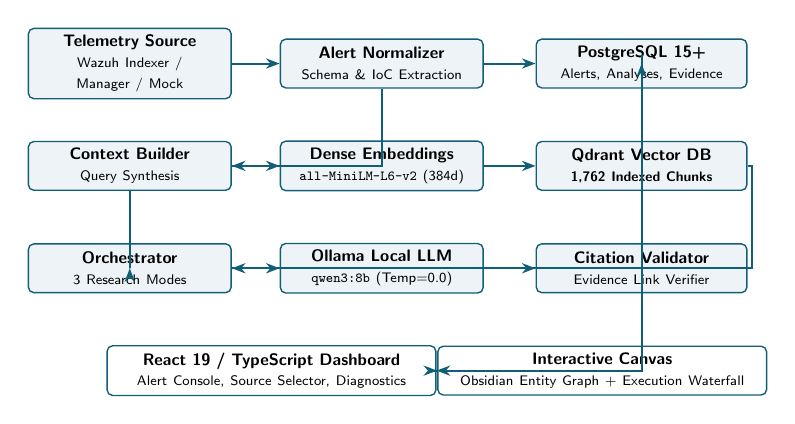
\begin{tikzpicture}[
  font=\sffamily\fontsize{6.5}{7.5}\selectfont,
  box/.style={rectangle, draw=SOCteal, fill=SOCpale, rounded corners=2pt, text centered, inner sep=2.5pt, line width=0.5pt, minimum height=0.62cm},
  arrow/.style={-{Stealth[scale=0.8]}, line width=0.7pt, color=SOCteal}
]
  % Row 1: Ingestion Tier
  \node[box, text width=2.4cm] (wazuh) at (0,2.5) {\textbf{Telemetry Source}\\ \tiny Wazuh Indexer / Manager / Mock};
  \node[box, text width=2.4cm] (norm) at (3.2,2.5) {\textbf{Alert Normalizer}\\ \tiny Schema \& IoC Extraction};
  \node[box, text width=2.5cm] (pg) at (6.5,2.5) {\textbf{PostgreSQL 15+}\\ \tiny Alerts, Analyses, Evidence};

  % Row 2: RAG Intelligence Tier
  \node[box, text width=2.4cm] (ctx) at (0,1.2) {\textbf{Context Builder}\\ \tiny Query Synthesis};
  \node[box, text width=2.4cm] (embed) at (3.2,1.2) {\textbf{Dense Embeddings}\\ \tiny \texttt{all-MiniLM-L6-v2} (384d)};
  \node[box, text width=2.5cm] (qdrant) at (6.5,1.2) {\textbf{Qdrant Vector DB}\\ \tiny \textbf{1,762 Indexed Chunks}};

  % Row 3: Reasoning & Validation Tier
  \node[box, text width=2.4cm] (orch) at (0,-0.1) {\textbf{Orchestrator}\\ \tiny 3 Research Modes};
  \node[box, text width=2.4cm] (llm) at (3.2,-0.1) {\textbf{Ollama Local LLM}\\ \tiny \texttt{qwen3:8b} (Temp=0.0)};
  \node[box, text width=2.5cm] (val) at (6.5,-0.1) {\textbf{Citation Validator}\\ \tiny Evidence Link Verifier};

  % Row 4: Presentation Tier
  \node[box, text width=4.0cm, fill=white] (ui) at (1.8,-1.4) {\textbf{React 19 / TypeScript Dashboard}\\ \tiny Alert Console, Source Selector, Diagnostics};
  \node[box, text width=4.0cm, fill=white] (graph) at (6.0,-1.4) {\textbf{Interactive Canvas}\\ \tiny Obsidian Entity Graph + Execution Waterfall};

  % Connectors
  \draw[arrow] (wazuh) -- (norm);
  \draw[arrow] (norm) -- (pg);
  \draw[arrow] (norm) |- (ctx);
  \draw[arrow] (ctx) -- (embed);
  \draw[arrow] (embed) -- (qdrant);
  \draw[arrow] (ctx) |- (orch);
  \draw[arrow] (qdrant) -- ++(1.4,0) |- (orch);
  \draw[arrow] (orch) -- (llm);
  \draw[arrow] (llm) -- (val);
  \draw[arrow] (val) |- (pg);
  \draw[arrow] (pg) |- (ui);
  \draw[arrow] (ui) -- (graph);
\end{tikzpicture}
\end{center}

\vspace{-0.1cm}
\begin{columns}[T,onlytextwidth]
\column{0.32\textwidth}
\SOCbox{\linewidth}{SOCline}{SOCpale}{\tiny\textbf{Ingestion:} Multi-source isolation stamps demo vs. live telemetry.}
\column{0.32\textwidth}
\SOCbox{\linewidth}{SOCline}{SOCpale}{\tiny\textbf{Knowledge:} 1,618 MITRE ATT\&CK + 144 NVD CVE vector chunks.}
\column{0.32\textwidth}
\SOCbox{\linewidth}{SOCline}{SOCpale}{\tiny\textbf{Privacy:} 100\% on-premise execution with zero external cloud leakage.}
\end{columns}
}

% =============================================================================
% SLIDE 4: System/Design Development: Request & Data Flow
% =============================================================================
\SOCslide{1. System/Design Development}{End-to-End Alert Ingestion and Evidence Processing Pipeline}{
\begin{columns}[T,onlytextwidth]
\column{0.60\textwidth}
\SOCcard{\linewidth}{6-Stage Sequential Operational Pipeline}{
\begin{enumerate}\setlength{\itemsep}{2pt}\scriptsize
  \item \textbf{Ingestion \& Normalization}: Parses Wazuh JSON/Syslog into normalized schema; extracts timestamps, agent, rule ID, and network IoCs.
  \item \textbf{Context Extraction \& Query Synthesis}: Synthesizes 3 targeted queries: rule text query, MITRE technique anchor, and entity context.
  \item \textbf{Dense Semantic Search (Qdrant)}: Computes 384-d cosine similarity over 1,762 chunks; retrieves top-$k$ evidence cards.
  \item \textbf{Evidence-Constrained Prompting}: Formats prompt with strict system instructions prohibiting uncited assertions.
  \item \textbf{Deterministic LLM Reasoning}: Local \texttt{qwen3:8b} evaluates threat scenario and formulates triage recommendations.
  \item \textbf{Citation Integrity Verification}: Automated validator verifies cited evidence IDs match retrieved items before database write.
\end{enumerate}
}
\column{0.38\textwidth}
\SOCcard{\linewidth}{Stage Latency Instrumentation}{
\scriptsize
\textbf{Measured Pipeline Durations:}
\begin{itemize}\setlength{\itemsep}{1.5pt}
  \item Ingestion \& Parse: 1--5 ms
  \item Normalization \& DB: 2--8 ms
  \item MiniLM Embeddings: 30--60 ms
  \item Qdrant Vector Search: 8--25 ms
  \item Ollama Inference (\texttt{qwen3:8b}): 35--80 s
  \item Citation Validation: 1--3 ms
\end{itemize}
\vspace{2pt}
\textbf{\color{SOCteal}Integrity Guarantee:}\\
Uncited claims are flagged, ensuring transparent auditability for human analysts.
}
\end{columns}
}

% =============================================================================
% SLIDE 5: Implementation Progress: Subsystem Status & Services
% =============================================================================
\SOCslide{2. Implementation Progress}{Subsystem Development Status \& Infrastructure Overview}{
\begin{center}
\resizebox{0.96\textwidth}{!}{%
\begin{tabular}{l p{3.2cm} p{7.8cm} c}
\toprule
\textbf{Subsystem} & \textbf{Component Technology} & \textbf{Implementation Details \& Verification Evidence} & \textbf{Status} \\
\midrule
\textbf{Backend Core} & FastAPI (Python 3.11/13) & Asynchronous REST API, typed Pydantic V2 schemas, SSE trace streaming & \textcolor{SOCgreen}{\textbf{Verified}} \\
\textbf{Relational DB} & PostgreSQL 15+ / Alembic & Tables: \texttt{alerts} (95 records), \texttt{analyses} (44 records), \texttt{evidence} (48 records) & \textcolor{SOCgreen}{\textbf{Verified}} \\
\textbf{Vector DB} & Qdrant Engine (v1.18+) & Collection \texttt{security\_knowledge} active with \textbf{1,762 indexed vector points} & \textcolor{SOCgreen}{\textbf{Verified}} \\
\textbf{Embeddings} & \texttt{all-MiniLM-L6-v2} & 384-dimensional dense semantic vectors, local PyTorch inference & \textcolor{SOCgreen}{\textbf{Verified}} \\
\textbf{Local LLM} & Ollama / \texttt{qwen3:8b} & 8B parameter local reasoning at temperature 0.0; JSON schema enforcement & \textcolor{SOCgreen}{\textbf{Verified}} \\
\textbf{Frontend UI} & React 19 + TypeScript & Single-page app with Obsidian Entity Graph and Execution Waterfall traces & \textcolor{SOCgreen}{\textbf{Verified}} \\
\textbf{Source Manager} & Isolated 3-Mode Abstraction & Demo (active default), Live Wazuh (clean empty state), Dataset Replay & \textcolor{SOCgreen}{\textbf{Verified}} \\
\textbf{Wazuh Transport} & Indexer \& Manager Clients & Read-only OpenSearch DSL (\texttt{POST /wazuh-alerts-*/\_search}) \& JWT manager & \textcolor{SOCamber}{\textbf{Client Verified}} \\
\textbf{Deployment} & Docker Compose & Multi-service container orchestration with internal health probes & \textcolor{SOCgreen}{\textbf{Verified}} \\
\bottomrule
\end{tabular}%
}
\end{center}

\vspace{-0.05cm}
\SOCbox{0.96\textwidth}{SOCline}{SOCpale}{
  \scriptsize\textbf{Live Service Probe Verified (2026-10-26 13:16 IST):} \texttt{GET /health} $\to$ \texttt{dependencies\_ok: true}, PostgreSQL: connected (68ms), Qdrant: connected (1,762 points), Ollama: reachable (\texttt{qwen3:8b}).
}
}

% =============================================================================
% SLIDE 6: Implementation Progress: Frontend Workspaces & Features
% =============================================================================
\SOCslide{2. Implementation Progress}{Frontend SOC Workspaces and Interactive Visualization}{
\begin{columns}[T,onlytextwidth]
\column{0.48\textwidth}
\SOCcard{\linewidth}{Operational Analyst Modules}{
\begin{itemize}\setlength{\itemsep}{1.2pt}\scriptsize
  \item \textbf{SOC Executive Dashboard}: Real-time KPI summary, severity donut distribution (25 Critical, 52 High, 12 Medium, 6 Low), and component health matrix.
  \item \textbf{Alert Management Console}: Tabular alert stream with severity badges, pagination, status updates, and deep inspector links.
  \item \textbf{AI Investigation Workspace}: Multi-mode analysis triggering, structured threat synthesis, recommendations, and confidence indicator.
  \item \textbf{Data Source Selector}: Top command-bar segmented selector switching between Demo Data, Live Wazuh, and Replay.
\end{itemize}
}
\column{0.48\textwidth}
\SOCcard{\linewidth}{Advanced Analytical Workspaces}{
\begin{itemize}\setlength{\itemsep}{1.2pt}\scriptsize
  \item \textbf{Obsidian-Style Entity Graph}: Force-directed interactive canvas linking alerts, hostnames, IP addresses, usernames, and MITRE techniques (\texttt{EntityGraphPage.tsx}).
  \item \textbf{Pipeline Execution Waterfall}: Visual timeline inspector tracking per-stage latencies and intermediate outputs (\texttt{ExecutionTracesPage.tsx}).
  \item \textbf{Evaluation Benchmark UI}: Progress tracker displaying real-time metrics across test runs (\texttt{Evaluation.tsx}).
  \item \textbf{Honest Empty States}: Dedicated UI disclosure when Live Wazuh is selected without configured endpoints.
\end{itemize}
}
\end{columns}

\vspace{0.10cm}
\SOCbox{0.96\textwidth}{SOCline}{SOCpale}{
  \scriptsize\textbf{UI Verification Status:} \textbf{32 passed frontend unit tests} across 8 suites (Vitest v5.0.1); production build compiles cleanly in 4.91s.
}
}

% =============================================================================
% SLIDE 7: Implementation Progress: Rigorous Software Testing
% =============================================================================
\SOCslide{2. Implementation Progress}{Empirical Software Engineering Validation \& Test Coverage}{
\begin{columns}[T,onlytextwidth]
\column{0.48\textwidth}
\SOCcard{\linewidth}{Backend Test Suite (Pytest v9.1.1)}{
\begin{itemize}\setlength{\itemsep}{2pt}
  \item \textbf{Total Passed}: \textcolor{SOCgreen}{\textbf{226 Passed}}, 0 Failed (44.51s)
  \item \textbf{Environment}: Python 3.11/3.13 in Docker container
  \item \textbf{Verified Functional Domains}:
    \begin{itemize}\scriptsize
      \item Ingestion, deduplication \& persistence (5 tests)
      \item Data source isolation \& Indexer client (5 tests)
      \item Knowledge chunking \& embeddings (53 tests)
      \item Vector store indexing \& search (8 tests)
      \item Security context \& query extraction (28 tests)
      \item Orchestrator modes \& validation (27 tests)
      \item Evaluation metrics \& resume runner (33 tests)
      \item Wazuh transport \& HTTP client (15 tests)
    \end{itemize}
\end{itemize}
}
\column{0.48\textwidth}
\SOCcard{\linewidth}{Frontend Test Suite (Vitest v5.0.1)}{
\begin{itemize}\setlength{\itemsep}{1.2pt}\scriptsize
  \item \textbf{Total Passed}: \textcolor{SOCgreen}{\textbf{32 Passed}}, 0 Failed (27.01s)
  \item \textbf{Environment}: React 19, TypeScript, Vite
  \item \textbf{Verified Component Suites}:
    \begin{itemize}\scriptsize
      \item \texttt{Dashboard}: Metric rendering \& empty states
      \item \texttt{Alerts}: Filtering, search \& provenance chips
      \item \texttt{AIAnalysis}: Mode selection \& error recovery
      \item \texttt{EntityGraph}: Canvas interaction \& nodes
      \item \texttt{ExecutionTraces}: Waterfall \& drawer
      \item \texttt{Evaluation}: Benchmark run tracking
      \item \texttt{Layout}: Navigation \& source selector
      \item \texttt{App}: Router configuration \& fallbacks
    \end{itemize}
\end{itemize}
}
\end{columns}

\vspace{0.20cm}
\SOCbox{0.96\textwidth}{SOCline}{SOCpale}{
  \scriptsize\textbf{Research Honesty Distinction:} Software unit tests (258 total passed) validate code correctness and API contracts; they are strictly distinguished from threat detection accuracy evaluated on security benchmarks.
}
}

% =============================================================================
% SLIDE 8: Technical Approach: RAG, Embeddings & LLM Integration
% =============================================================================
\SOCslide{3. Technical Approach}{Evidence-Grounded RAG Pipeline and Threat Knowledge Integration}{
\begin{columns}[T,onlytextwidth]
\column{0.50\textwidth}
\SOCcard{\linewidth}{Knowledge Base Construction}{
\begin{itemize}\setlength{\itemsep}{2pt}
  \item \textbf{MITRE ATT\&CK Enterprise (v14)}: Extracted 1,618 techniques, tactics, mitigation steps, and detection guidelines.
  \item \textbf{NIST NVD CVE Security Feed}: Extracted 144 high-impact CVE entries with CVSS scores, affected software, and remediation paths.
  \item \textbf{Chunking \& Indexing}: 1,200 character chunks with 150 character overlap; indexed into Qdrant using 384-d cosine similarity.
  \item \textbf{Deterministic Embeddings}: Local \texttt{all-MiniLM-L6-v2} model running on CPU/GPU without cloud calls.
\end{itemize}
}
\column{0.50\textwidth}
\SOCcard{\linewidth}{Multi-Query Retrieval Strategy}{
\begin{itemize}\setlength{\itemsep}{2pt}
  \item \textbf{Rule Query}: Synthesizes query directly from alert rule description to identify relevant attack categories.
  \item \textbf{Technique Anchor}: Injects explicit MITRE technique tags from security context to anchor top-1 retrieval.
  \item \textbf{Entity Context}: Leverages host, user, and network indicators for targeted vulnerability correlation.
  \item \textbf{Strict Citation Validation}: Rejects or flags assertions lacking explicit evidence IDs.
\end{itemize}
}
\end{columns}

\vspace{0.25cm}
\SOCbox{0.96\textwidth}{SOCline}{SOCpale}{
  \scriptsize\textbf{Parametric vs. Retrieved Knowledge:} Without RAG, LLMs rely on outdated training memory; grounding retrieval in Qdrant ensures recommendations reflect verified security frameworks.
}
}

% =============================================================================
% SLIDE 9: Technical Approach: Multi-Source Architecture & Wazuh Integration
% =============================================================================
\SOCslide{3. Technical Approach}{Data-Source Abstraction and Read-Only Wazuh Connector}{
\begin{columns}[T,onlytextwidth]
\column{0.48\textwidth}
\SOCcard{\linewidth}{Three Strictly Isolated Data Sources}{
\begin{itemize}\setlength{\itemsep}{2pt}
  \item \textbf{Mode 1 --- Demo (\texttt{demo})}: 95 persistent records (52 attack scenario alerts, 40 benchmark cases). Serves as dashboard and evaluation baseline.
  \item \textbf{Mode 2 --- Live Wazuh (\texttt{live\_wazuh})}: Real alerts from configured Wazuh Indexer or Manager. Displays 0 alerts and honest empty state until connected.
  \item \textbf{Mode 3 --- Dataset Replay (\texttt{dataset\_replay})}: Offline benchmark datasets (e.g. CIC-IDS2017); explicitly labeled as historical replay.
\end{itemize}
}
\column{0.48\textwidth}
\SOCcard{\linewidth}{Wazuh Connector Design}{
\begin{itemize}\setlength{\itemsep}{2pt}
  \item \textbf{Preferred: Wazuh Indexer API}: Queries OpenSearch cluster directly (\texttt{POST /wazuh-alerts-*/\_search}) over TLS with HTTP Basic Auth.
  \item \textbf{Wazuh Manager API}: REST API client with automatic JWT token acquisition and refresh (\texttt{GET /alerts}).
  \item \textbf{Read-Only Guarantees}: Connectors perform zero write, delete, or re-indexing operations on remote Wazuh deployments.
  \item \textbf{Credential Isolation}: All secrets stored in \texttt{.env}; never committed or exposed in UI bundles.
\end{itemize}
}
\end{columns}

\vspace{0.20cm}
\SOCbox{0.96\textwidth}{SOCline}{SOCpale}{
  \scriptsize\textbf{Integrity Safeguard:} The backend never mixes demo and live records, never inflates live counters, and provides honest UI status when unconfigured.
}
}

% =============================================================================
% SLIDE 10: Technical Approach: Evaluation Protocol & Methodology
% =============================================================================
\SOCslide{3. Technical Approach}{Controlled Tri-Mode Evaluation Protocol \& Quantitative Metrics}{
\begin{columns}[T,onlytextwidth]
\column{0.48\textwidth}
\SOCcard{\linewidth}{Controlled 3-Mode Experiment Design}{
\begin{itemize}\setlength{\itemsep}{2pt}
  \item \textbf{Mode 1 (\texttt{llm\_only})}: Baseline. Alert passed to \texttt{qwen3:8b} without external retrieval; measures raw model memory.
  \item \textbf{Mode 2 (\texttt{standard\_rag})}: Unanchored semantic search using rule description text; tests basic vector retrieval.
  \item \textbf{Mode 3 (\texttt{evidence\_aware})}: Multi-query synthesis, entity anchoring, top-$k$ evidence ranking, and strict citation verification.
\end{itemize}
}
\column{0.48\textwidth}
\SOCcard{\linewidth}{Evaluation Datasets \& Scenarios}{
\begin{itemize}\setlength{\itemsep}{2pt}
  \item \textbf{Dataset v1 (Smoke Baseline)}: 8 multi-stage scenarios across brute-force, web attacks, and privilege escalation.
  \item \textbf{Dataset v2 (Benchmark)}: 40 curated scenarios across 7 attack categories + benign controls ($40 \times 3 = 120$ planned evaluations).
  \item \textbf{Benign Control Scenarios}: Evaluates false alarm resistance on routine administrative events.
\end{itemize}
}
\end{columns}

\vspace{0.25cm}
\SOCbox{0.96\textwidth}{SOCline}{SOCpale}{
  \scriptsize\textbf{Evaluated Metric Suite:} Technique Precision/Recall/F1, CVE Precision/Recall/F1, Valid Citation Rate, Retrieval Recall@1, Recall@5, MRR, Wall Latency, and LLM Inference Latency.
}
}

% =============================================================================
% SLIDE 11: Preliminary Results: Empirical Benchmark Findings
% =============================================================================
\SOCslide{4. Preliminary Results}{Empirical Findings from Controlled Benchmark Runs}{
\SOCbox{0.96\textwidth}{SOCamber}{SOCpale}{
  \scriptsize\textbf{Benchmark Execution Status (Dataset v2, Run \texttt{20261024-145621-1345d6}):}
  40 scenarios $\times$ 3 modes = 120 planned evaluations. Currently \textbf{12 scenarios completed (36 evaluations completed)}, with 84 evaluations pending execution.
}

\vspace{0.15cm}
\begin{center}
\resizebox{0.96\textwidth}{!}{%
\begin{tabular}{l c c c c c c}
\toprule
\textbf{Evaluation Mode} & \textbf{Cases ($N$)} & \textbf{Avg Wall Latency} & \textbf{Technique Prec.} & \textbf{Technique Recall} & \textbf{Technique F1} & \textbf{Valid Citation Rate} \\
\midrule
\textbf{LLM-Only (Baseline)} & 12 & 36.8 s & 0.500 & 0.417 & 0.444 & N/A (no citations) \\
\textbf{Standard RAG} & 12 & 82.2 s & 0.500 & 0.417 & 0.444 & \textbf{1.000 (100\%)} \\
\textbf{Evidence-Aware RAG} & 12 & 79.6 s & 0.500 & 0.417 & 0.444 & \textbf{1.000 (100\%)} \\
\bottomrule
\end{tabular}%
}
\end{center}

\vspace{0.15cm}
\begin{columns}[T,onlytextwidth]
\column{0.48\textwidth}
\SOCcard{\linewidth}{Dataset v1 Baseline ($N=8$, Completed)}{
\begin{itemize}\setlength{\itemsep}{1.5pt}\scriptsize
  \item \textbf{Retrieval Recall@1}: \textbf{1.000} (Evidence-Aware) vs \textbf{0.250} (Standard RAG) vs 0.000 (LLM-Only).
  \item \textbf{Retrieval MRR}: \textbf{1.000} vs \textbf{0.354} for Standard RAG.
  \item \textbf{Technique F1}: 0.833 across 8 smoke scenarios.
\end{itemize}
}
\column{0.48\textwidth}
\SOCcard{\linewidth}{Retrieval-Only Ablation (No LLM)}{
\begin{itemize}\setlength{\itemsep}{1.5pt}\scriptsize
  \item \textbf{Semantic Anchored}: Recall@1 = \textbf{1.000}, MRR = \textbf{1.000} (1563 ms).
  \item \textbf{Semantic Unanchored}: Recall@1 = 0.375, MRR = 0.463 (338 ms).
  \item \textbf{Key Takeaway}: Entity anchoring dramatically improves top-1 retrieval accuracy.
\end{itemize}
}
\end{columns}
}

% =============================================================================
% SLIDE 12: Technical Limitations & Challenges
% =============================================================================
\SOCslide{Limitations \& Challenges}{Transparent Analysis of Current Engineering Constraints}{
\begin{columns}[T,onlytextwidth]
\column{0.48\textwidth}
\SOCcard{\linewidth}{Identified Technical Limitations}{
\begin{itemize}\setlength{\itemsep}{3pt}
  \item \textbf{Simulated Evaluation Scenarios}: Benchmarks currently utilize curated synthetic scenarios; validation on noisy enterprise production logs remains ongoing.
  \item \textbf{Inference Latency on Local Hardware}: Local \texttt{qwen3:8b} inference requires 35--80s per alert on host hardware; presents challenges for real-time high-throughput triage.
  \item \textbf{Pending Live Wazuh Deployment}: Wazuh Indexer and Manager client code is fully verified, but evaluation currently operates in mock mode due to host memory constraints (16GB RAM).
\end{itemize}
}
\column{0.48\textwidth}
\SOCcard{\linewidth}{Integrity \& Engineering Mitigations}{
\begin{itemize}\setlength{\itemsep}{3pt}
  \item \textbf{Checkpoint Resume Protocol}: Evaluator saves intermediate state to \texttt{results\_partial.json}, preventing data loss on interrupted runs.
  \item \textbf{Explicit UI Disclaimers}: Prominent badge disclosures inform analysts of mock/synthetic data mode.
  \item \textbf{Exact vs. Semantic Scoring}: Current scorer requires exact MITRE ID matches; related parent techniques receive zero credit, representing conservative lower-bound metrics.
\end{itemize}
}
\end{columns}
}

% =============================================================================
% SLIDE 13: Future Work & Next Milestones
% =============================================================================
\SOCslide{Future Work \& Next Milestones}{Planned Research Activities for Final Review}{
\begin{center}
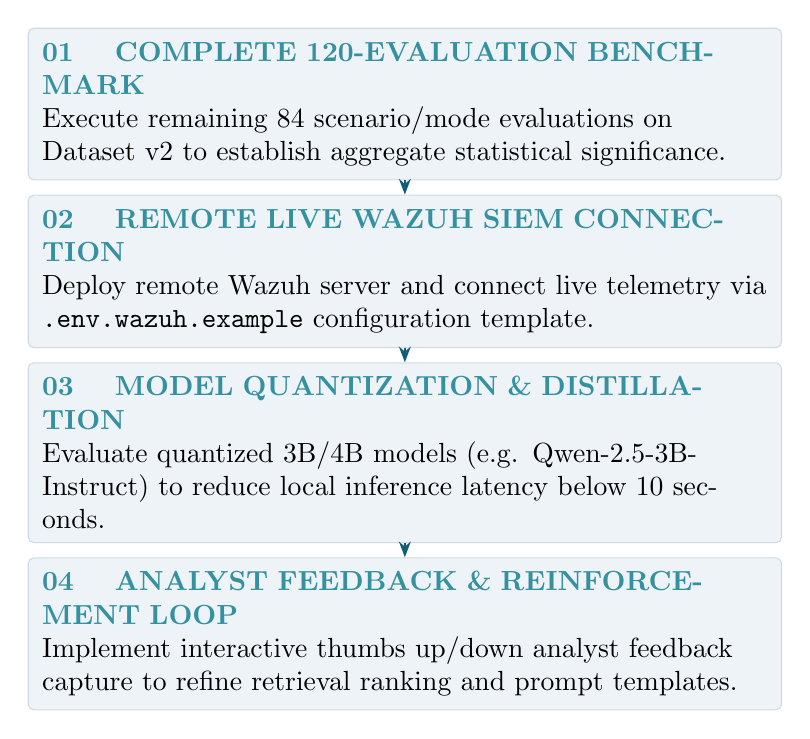
\begin{tikzpicture}[node distance=0.18cm]
\node[draw=SOCline,fill=SOCpale,rounded corners=2pt,text width=0.76\textwidth,inner sep=5pt] (a)
{\textbf{\color{SOCtealLight}01 \quad COMPLETE 120-EVALUATION BENCHMARK}\\Execute remaining 84 scenario/mode evaluations on Dataset v2 to establish aggregate statistical significance.};

\node[draw=SOCline,fill=SOCpale,rounded corners=2pt,text width=0.76\textwidth,inner sep=5pt,below=of a] (b)
{\textbf{\color{SOCtealLight}02 \quad REMOTE LIVE WAZUH SIEM CONNECTION}\\Deploy remote Wazuh server and connect live telemetry via \texttt{.env.wazuh.example} configuration template.};

\node[draw=SOCline,fill=SOCpale,rounded corners=2pt,text width=0.76\textwidth,inner sep=5pt,below=of b] (c)
{\textbf{\color{SOCtealLight}03 \quad MODEL QUANTIZATION \& DISTILLATION}\\Evaluate quantized 3B/4B models (e.g. Qwen-2.5-3B-Instruct) to reduce local inference latency below 10 seconds.};

\node[draw=SOCline,fill=SOCpale,rounded corners=2pt,text width=0.76\textwidth,inner sep=5pt,below=of c] (d)
{\textbf{\color{SOCtealLight}04 \quad ANALYST FEEDBACK \& REINFORCEMENT LOOP}\\Implement interactive thumbs up/down analyst feedback capture to refine retrieval ranking and prompt templates.};

\foreach \x/\y in {a/b,b/c,c/d}
  \draw[-{Stealth[length=2mm]},SOCteal,line width=0.8pt] (\x.south)--(\y.north);
\end{tikzpicture}
\end{center}
}

% =============================================================================
% SLIDE 14: Conclusion & Summary of Deliverables
% =============================================================================
\SOCslide{Conclusion}{Summary of Achieved Milestones for PPD-II Second Review}{
\begin{columns}[T,onlytextwidth]
\column{0.55\textwidth}
\SOCcard{\linewidth}{Summary of Review Deliverables}{
\begin{itemize}\setlength{\itemsep}{3pt}
  \item \textbf{System/Design Development}: Architected a fully containerized, multi-tier SOC Assistant integrating PostgreSQL, Qdrant, and Ollama.
  \item \textbf{Technical Approach}: Engineered an evidence-aware RAG pipeline indexing 1,762 MITRE ATT\&CK and NVD chunks with strict citation validation.
  \item \textbf{Implementation Progress}: Developed React 19 UI with Entity Graph and Waterfall traces, verified by \textbf{226 backend and 32 frontend unit tests}.
  \item \textbf{Preliminary Results}: Established 100\% valid citation integrity and demonstrated superior top-1 retrieval precision (Recall@1 = 1.0 vs 0.25).
\end{itemize}
}
\column{0.41\textwidth}
\begin{tcolorbox}[colback=SOCteal,colframe=SOCteal,arc=2mm,center,top=8pt,bottom=8pt]
  \centering
  \textcolor{white}{\large\textbf{Thank You!}}\\[6pt]
  \textcolor{SOCtealLight!40}{\footnotesize\textbf{Questions \& Discussion}}\\[10pt]
  \textcolor{white!90}{\scriptsize Kunal Sanga \quad\textbar\quad Reg: 2301341031}\\
  \textcolor{white!80}{\scriptsize Department of CSE}\\
  \textcolor{white!70}{\scriptsize Silicon Institute of Technology, Sambalpur}
\end{tcolorbox}
\vspace{0.15cm}
\SOCbox{\linewidth}{SOCline}{SOCpale}{
  \scriptsize\centering\textbf{Status:} PPD-II Second Review Completed
}
\end{columns}
}

% =============================================================================
% SLIDE 15: References
% =============================================================================
\SOCslide{References}{Academic Literature and Standard Threat Intelligence Frameworks}{
\footnotesize
\begin{enumerate}\setlength{\itemsep}{5pt}
  \item Ismail et al., ``Enhancing Security Operations Center: Wazuh Security Event Response with Retrieval-Augmented-Generation-Driven Copilot'', \textit{Sensors}, 2025.
  \item Habibzadeh, Feyzi \& Ebrahimi Atani, ``Large Language Models for Security Operations Centers: A Comprehensive Survey'', \textit{Journal of Electrical and Computer Engineering}, 2026.
  \item Taysi et al., ``Evidence-First Retrieval Augmented Generation with Claim Repair for Security Operations Center Workflows'', \textit{IEEE ICHORA}, 2026.
  \item Hahn et al., ``Non-Disruptive Disruption: An Empirical Experience of Introducing LLMs in the SOC'', \textit{NDSS / Internet Society}, 2026.
  \item MITRE Corporation, ``MITRE ATT\&CK Enterprise Framework (Version 14)'', \url{https://attack.mitre.org/}, 2023.
  \item National Institute of Standards and Technology (NIST), ``National Vulnerability Database (NVD) Data Feeds'', \url{https://nvd.nist.gov/}, 2024.
\end{enumerate}
}

\end{document}